\documentclass[14pt]{extbook}
\usepackage{multicol, enumerate, enumitem, hyperref, color, soul, setspace, parskip, fancyhdr} %General Packages
\usepackage{amssymb, amsthm, amsmath, bbm, latexsym, units, mathtools} %Math Packages
\everymath{\displaystyle} %All math in Display Style
% Packages with additional options
\usepackage[headsep=0.5cm,headheight=12pt, left=1 in,right= 1 in,top= 1 in,bottom= 1 in]{geometry}
\usepackage[usenames,dvipsnames]{xcolor}
\usepackage{dashrule}  % Package to use the command below to create lines between items
\newcommand{\litem}[1]{\item#1\hspace*{-1cm}\rule{\textwidth}{0.4pt}}
\pagestyle{fancy}
\lhead{Progress Quiz 3}
\chead{}
\rhead{Version C}
\lfoot{3148-2249}
\cfoot{}
\rfoot{Spring 2021}
\begin{document}

\begin{enumerate}
\litem{
Solve the radical equation below. Then, choose the interval(s) that the solution(s) belongs to.\[ \sqrt{35 x^2 - 28} - \sqrt{-29 x} = 0 \]\begin{enumerate}[label=\Alph*.]
\item \( x \in [-2.1,-0.9] \)
\item \( \text{All solutions lead to invalid or complex values in the equation.} \)
\item \( x_1 \in [-1.2, 1] \text{ and } x_2 \in [1.38,1.75] \)
\item \( x_1 \in [-2.1, -0.9] \text{ and } x_2 \in [-0.08,0.79] \)
\item \( x \in [-1.2,1] \)

\end{enumerate} }
\litem{
What is the domain of the function below?\[ f(x) = \sqrt[7]{-3 x + 7} \]\begin{enumerate}[label=\Alph*.]
\item \( \text{The domain is } (-\infty, a], \text{   where } a \in [1.3, 4] \)
\item \( (-\infty, \infty) \)
\item \( \text{The domain is } (-\infty, a], \text{   where } a \in [0.3, 1.5] \)
\item \( \text{The domain is } [a, \infty), \text{   where } a \in [-0.43, 2.02] \)
\item \( \text{The domain is } [a, \infty), \text{   where } a \in [1.32, 2.45] \)

\end{enumerate} }
\litem{
Choose the graph of the equation below.\[ f(x) = \sqrt[3]{x - 10} + 7 \]\begin{enumerate}[label=\Alph*.]
\begin{multicols}{2}\item 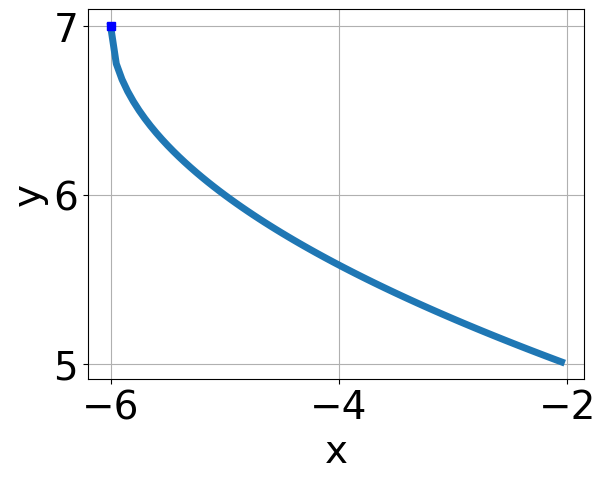
\includegraphics[width = 0.3\textwidth]{../Figures/radicalEquationToGraphAC.png}\item 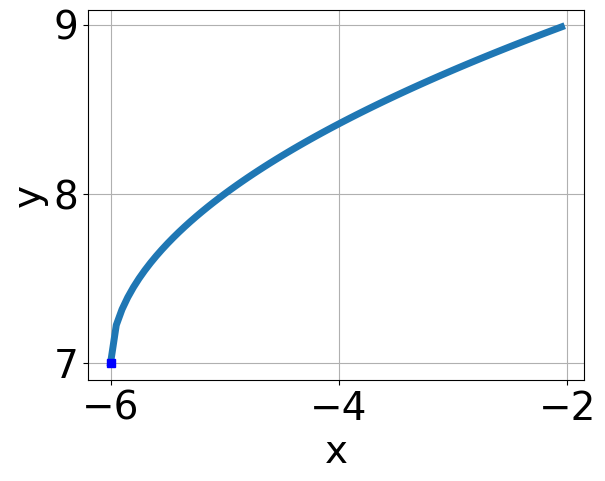
\includegraphics[width = 0.3\textwidth]{../Figures/radicalEquationToGraphBC.png}\item 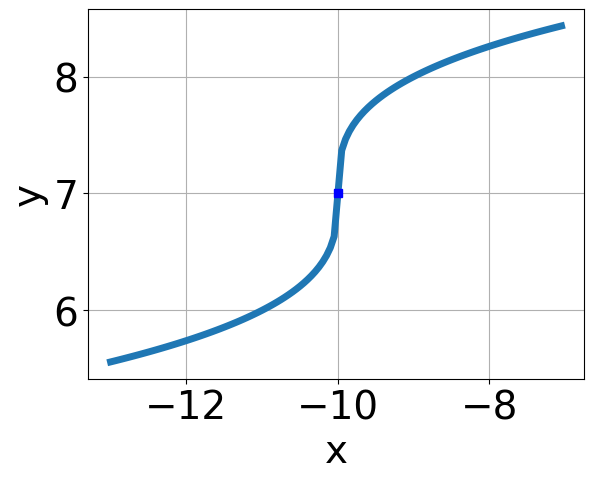
\includegraphics[width = 0.3\textwidth]{../Figures/radicalEquationToGraphCC.png}\item 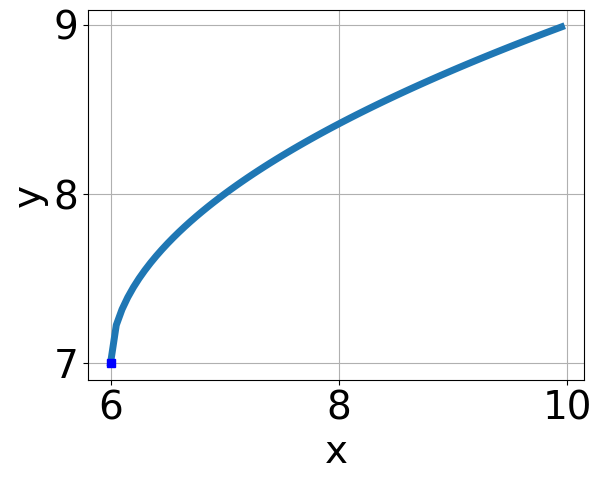
\includegraphics[width = 0.3\textwidth]{../Figures/radicalEquationToGraphDC.png}\end{multicols}\item None of the above.
\end{enumerate} }
\litem{
Choose the graph of the equation below.\[ f(x) = \sqrt[3]{x - 12} + 7 \]\begin{enumerate}[label=\Alph*.]
\begin{multicols}{2}\item 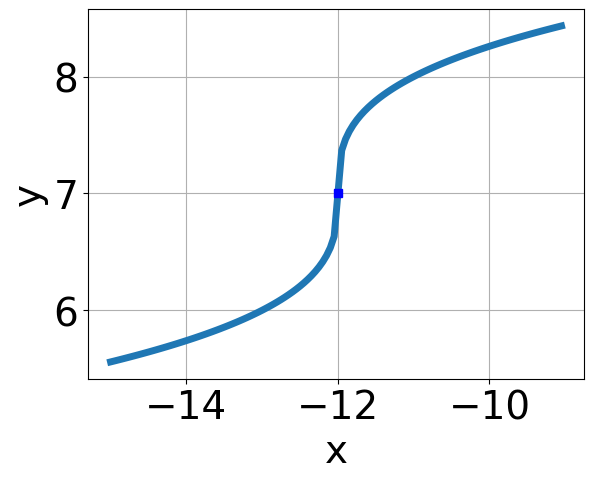
\includegraphics[width = 0.3\textwidth]{../Figures/radicalEquationToGraphCopyAC.png}\item 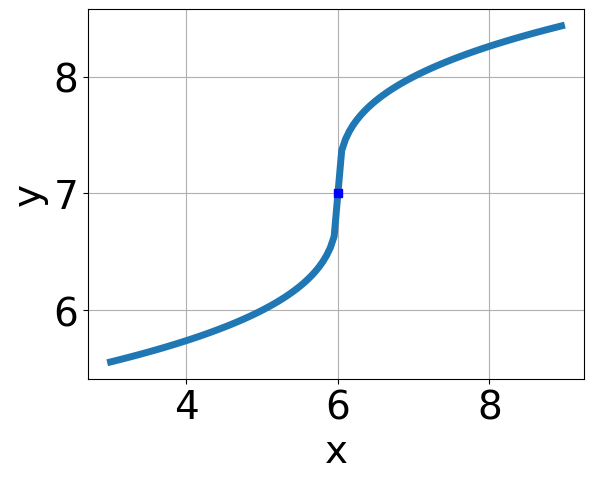
\includegraphics[width = 0.3\textwidth]{../Figures/radicalEquationToGraphCopyBC.png}\item 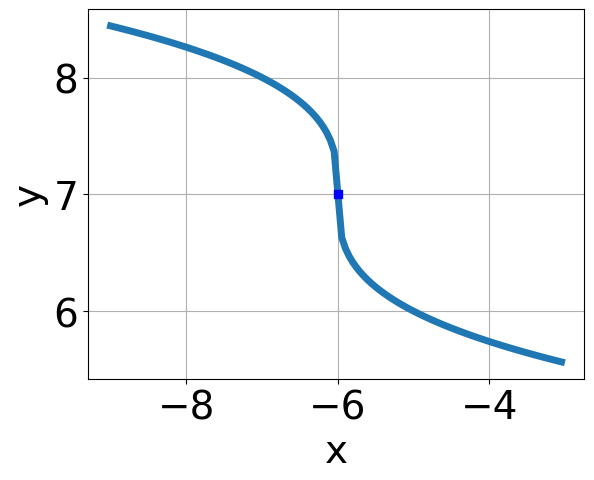
\includegraphics[width = 0.3\textwidth]{../Figures/radicalEquationToGraphCopyCC.png}\item 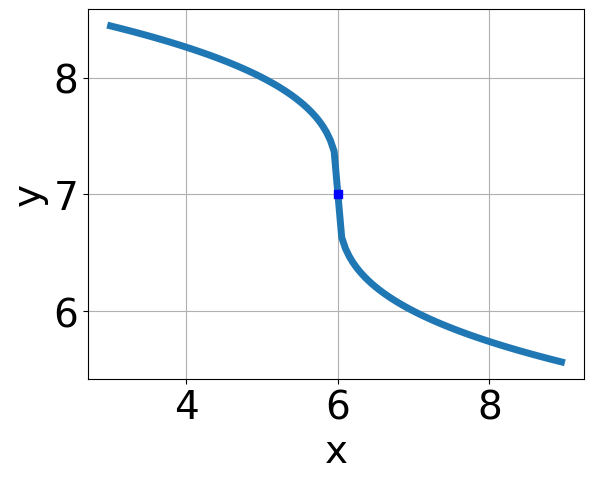
\includegraphics[width = 0.3\textwidth]{../Figures/radicalEquationToGraphCopyDC.png}\end{multicols}\item None of the above.
\end{enumerate} }
\litem{
Solve the radical equation below. Then, choose the interval(s) that the solution(s) belongs to.\[ \sqrt{72 x^2 - 21} - \sqrt{29 x} = 0 \]\begin{enumerate}[label=\Alph*.]
\item \( x_1 \in [-0.2, 0.71] \text{ and } x_2 \in [-1.22,3.78] \)
\item \( x \in [0.44,0.96] \)
\item \( x \in [-0.7,0.08] \)
\item \( \text{All solutions lead to invalid or complex values in the equation.} \)
\item \( x_1 \in [-0.7, 0.08] \text{ and } x_2 \in [-1.22,3.78] \)

\end{enumerate} }
\litem{
Solve the radical equation below. Then, choose the interval(s) that the solution(s) belongs to.\[ \sqrt{-7 x + 8} - \sqrt{-3 x - 4} = 0 \]\begin{enumerate}[label=\Alph*.]
\item \( x \in [0.71,1.13] \)
\item \( x_1 \in [1.08, 1.62] \text{ and } x_2 \in [1.6,4.6] \)
\item \( x_1 \in [-1.53, -0.79] \text{ and } x_2 \in [0,1.6] \)
\item \( \text{All solutions lead to invalid or complex values in the equation.} \)
\item \( x \in [2.73,3.15] \)

\end{enumerate} }
\litem{
What is the domain of the function below?\[ f(x) = \sqrt[3]{4 x + 7} \]\begin{enumerate}[label=\Alph*.]
\item \( (-\infty, \infty) \)
\item \( \text{The domain is } (-\infty, a], \text{   where } a \in [-2.3, -1.18] \)
\item \( \text{The domain is } (-\infty, a], \text{   where } a \in [-1.58, 0.74] \)
\item \( \text{The domain is } [a, \infty), \text{   where } a \in [-2.07, -1.73] \)
\item \( \text{The domain is } [a, \infty), \text{   where } a \in [-1.48, -0.38] \)

\end{enumerate} }
\litem{
Choose the equation of the function graphed below.
\begin{center}
    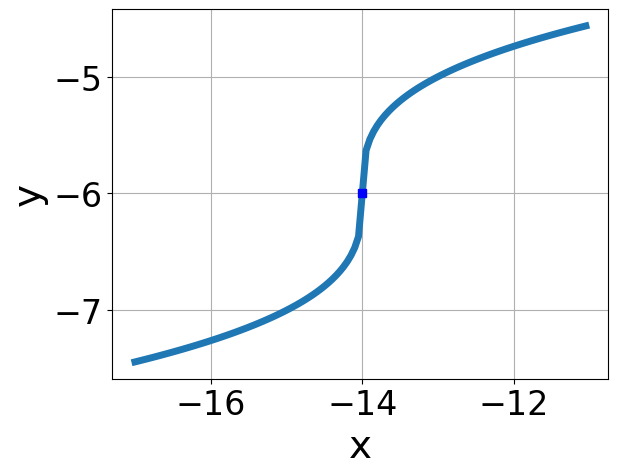
\includegraphics[width=0.5\textwidth]{../Figures/radicalGraphToEquationCopyC.png}
\end{center}
\begin{enumerate}[label=\Alph*.]
\item \( f(x) = - \sqrt{x - 14} + 3 \)
\item \( f(x) = \sqrt{x + 14} + 3 \)
\item \( f(x) = \sqrt{x - 14} + 3 \)
\item \( f(x) = - \sqrt{x + 14} + 3 \)
\item \( \text{None of the above} \)

\end{enumerate} }
\litem{
Choose the equation of the function graphed below.
\begin{center}
    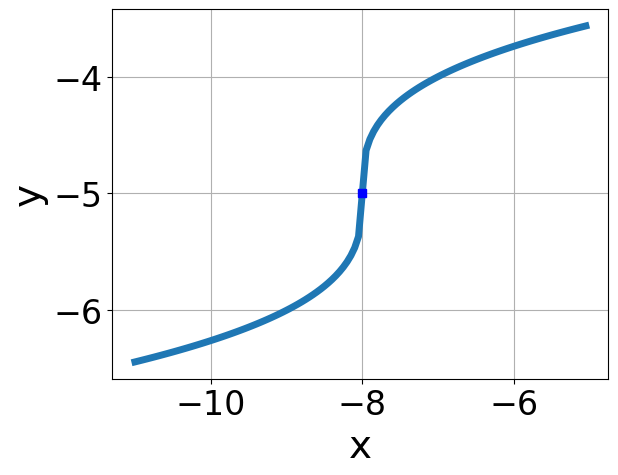
\includegraphics[width=0.5\textwidth]{../Figures/radicalGraphToEquationC.png}
\end{center}
\begin{enumerate}[label=\Alph*.]
\item \( f(x) = \sqrt{x - 8} - 4 \)
\item \( f(x) = - \sqrt{x + 8} - 4 \)
\item \( f(x) = - \sqrt{x - 8} - 4 \)
\item \( f(x) = \sqrt{x + 8} - 4 \)
\item \( \text{None of the above} \)

\end{enumerate} }
\litem{
Solve the radical equation below. Then, choose the interval(s) that the solution(s) belongs to.\[ \sqrt{-9 x + 2} - \sqrt{-7 x - 4} = 0 \]\begin{enumerate}[label=\Alph*.]
\item \( x \in [-1.58,-0.64] \)
\item \( \text{All solutions lead to invalid or complex values in the equation.} \)
\item \( x \in [2.37,3.34] \)
\item \( x_1 \in [-0.61, -0.19] \text{ and } x_2 \in [-0.78,2.22] \)
\item \( x_1 \in [-0.22, 0.49] \text{ and } x_2 \in [2,10] \)

\end{enumerate} }
\end{enumerate}

\end{document}